\documentclass[a4paper]{article}
\usepackage[utf8]{inputenc}
\usepackage{graphicx}
\graphicspath{ {./images/} }

\title{Projektskizze: WLAN-AP mit regelmäßigem PSK-Tausch und RFID-Anmeldung}
\date{\today}

\begin{document}
	\maketitle
	
	
	\section{Problem}
	Der pre-shared Key eines WLAN-Netzwerkes wird in den meisten Heimnetzwerken einmal oder gar nicht geändert. Dies hat zur Folge, dass sobald einmal das Passwort geknackt oder bewusst/unbewusst weitergegeben wurde, sich jeder mit dem Access-Point verbinden kann. Regelmäßiges Wechseln des Keys führt, aber zu unangenehmen Mehraufwand, den sehr viele Nutzer nicht eingehen wollen. Die Folge sind ungewollte Endgeräte im eigenen Heimnetz.
	
	\section{Lösungsansätze}
	Ein RFID-Transponder übermittelt den wöchentlich wechselnden pre-shared Key. Mit diesem können sich Endgeräte anmelden und kommunizieren. Hiermit wird das Problem der ungewollten Nutzern gelöst, denn diese können sich sobald der Key gewechselt hat, nicht mehr im Netz anmelden. Zusätzlich wird der Key an einem Display angezeigt, damit sich auch Geräte ohne RFID mit dem Netz verbinden kann. Der RFID-Transponder und das Display sind mit einem RaspberryPi verbunden dieser dient als WLAN-Access-Point für das Netz und wird mit dem Router per LAN-Kabel verbunden.
	
	\section{Hardware}
	
	\begin{itemize}
		\item RaspberryPi
		\item Display
		\item RFID/NFC-Transponder
	\end{itemize}

	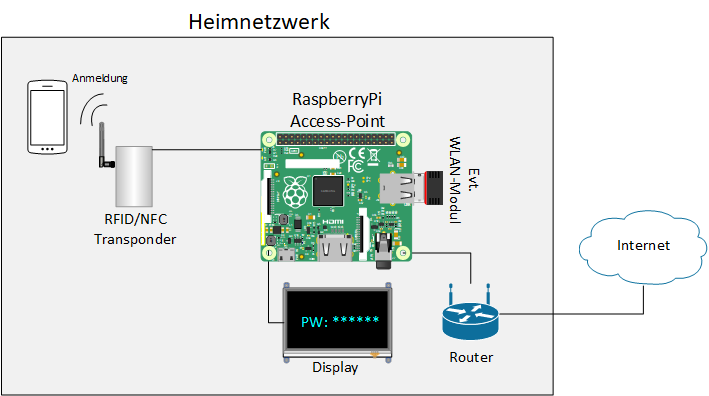
\includegraphics[scale=0.6]{skizze}

\end{document}
